\documentclass[11pt]{article}
\usepackage[utf8]{inputenc}
\usepackage{centernot}
\usepackage[parfill]{parskip}
\usepackage{amsmath}
\usepackage{amssymb}
\usepackage{graphicx}
\begin{document}
\title{Analys Problem 7}
\author{Robin Boregrim}
\maketitle
\renewcommand{\contentsname}{Innehållsförteckning}
\tableofcontents
\newpage
\section{Uppgiften}
Beräkna dubbelintegralen $$\iint_D \sin(\sqrt{x^2 + y^2})\textbf{ } dxdy$$
där $D$ är det område som bestäms av olikheterna $0<y<x$ \\
och $\pi^2 < x^2 + y^2 < 4\pi^2$.
\section{Lösning}
För att lätare lösa problemet så gör vi ett variabel byte till polära koordinater. Vi vill då få en dubbelintegral som beror på variablerna $r$och $\theta$ där 

$$\left\{\begin{array}{c}
r = \sqrt{x^2 + y^2}\\
x = r \sin \theta\\
y = r \cos  \theta
\end{array}\right. $$

Vi skriver om dubbelintegralen med de nya variablerna  $$\iint_D \sin(\sqrt{x^2 + y^2})\textbf{ } dxdy = \iint_E \sin(r)r\textbf{ }drd\theta .$$
Sen behöver vi beräkna gränerna för dessa variabler.\\
Gränserna för $r$ kan beräknas på följande sätt
$$\pi^2 < x^2 + y^2 < 4\pi^2 \Leftrightarrow$$$$ \pi^2 < r^2 < 4\pi^2 \Leftrightarrow $$$$ \pi < r < 2\pi$$
Eftersom att $r$ är roten av summan av två kvadrater behöver vi inte ta hänsyn till några negativa värden för $r$.\\
Gränserna till $\theta$ kan beräknas igenom att observera olikheten 
$$0<y<x.$$
Där kan vi se att y är begränsad av kurvorna $y = 0$ och $y = x$.
$$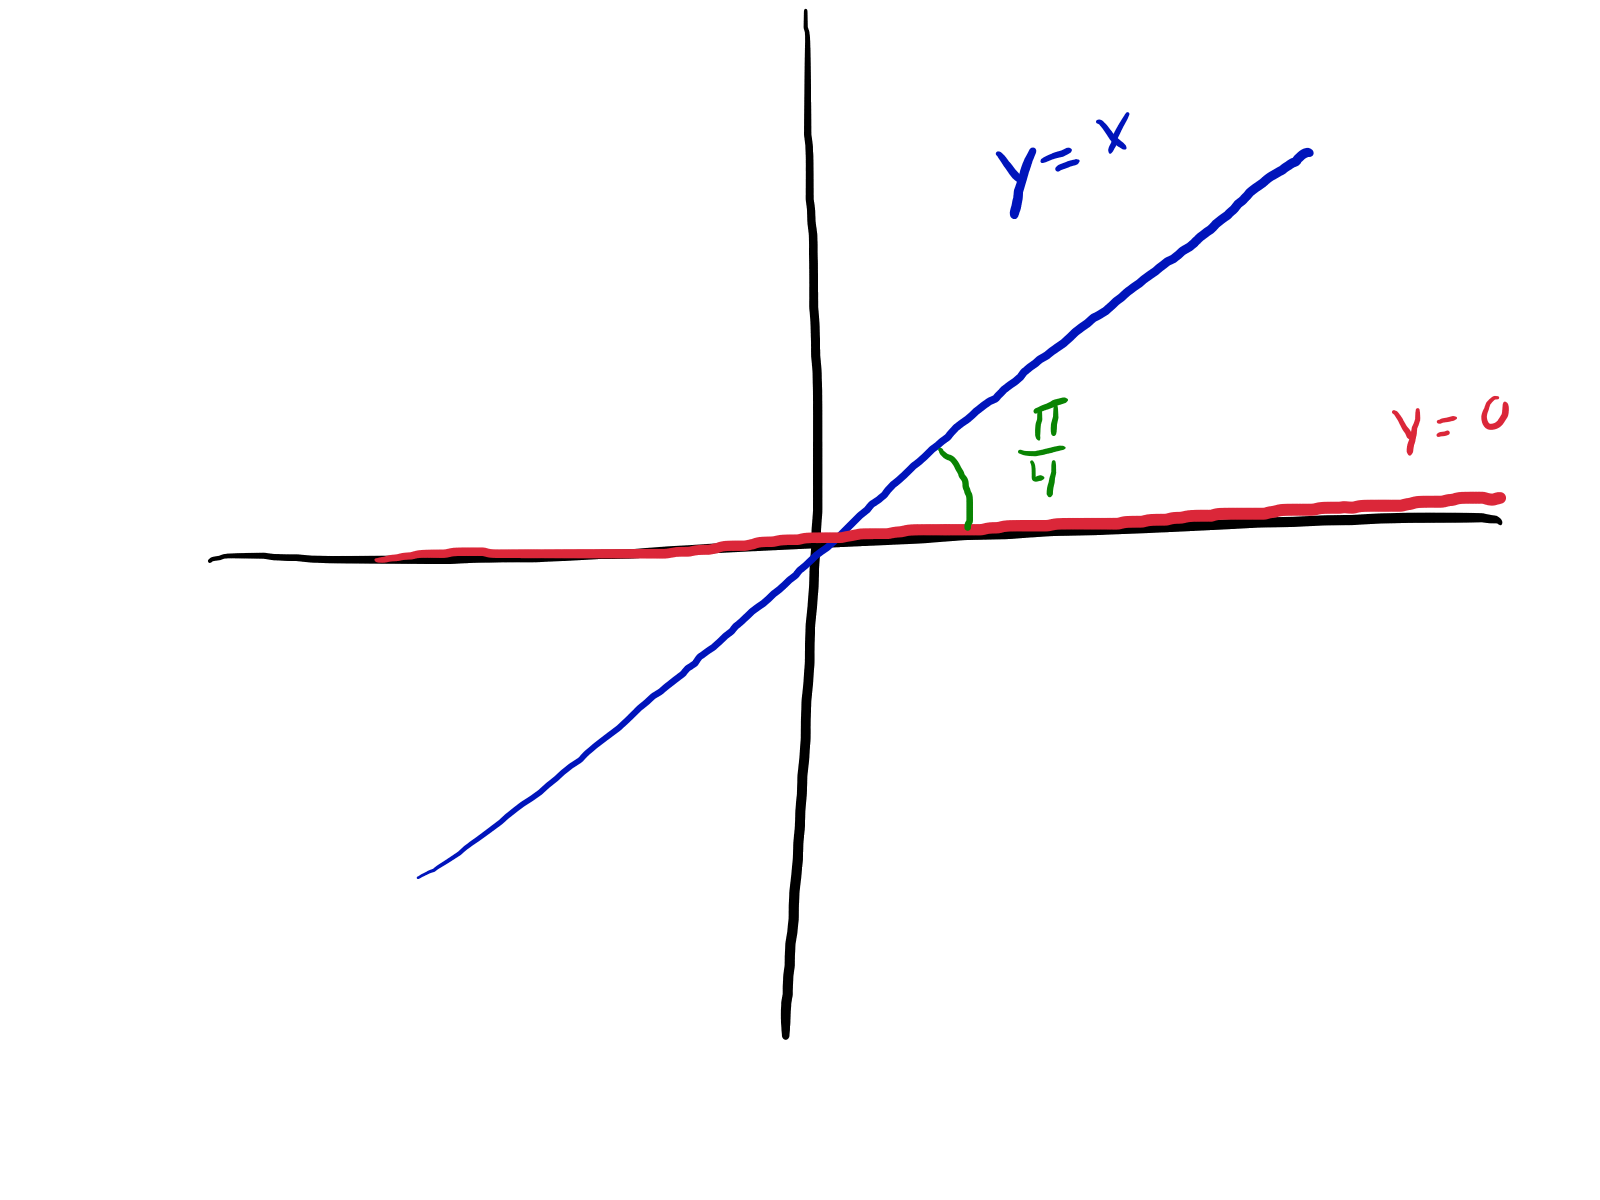
\includegraphics{Fig1.png}$$
Vinkeln för $y = x$ är $\frac{\pi}{4}$, detta betyder att gränserna för $\theta$ är $$0<\theta<\frac{\pi}{4}.$$
Vi kan nu beräkna dubbel integralen.
$$\iint_E \sin(r)r\textbf{ }drd\theta =$$
$$\int_{\pi}^{2\pi} \Bigg(\int_{0}^{\frac{\pi}{4}} \sin(r)r \textbf{ } d\theta\Bigg)dr =$$
$$\int_{\pi}^{2\pi}  \sin(r)r \Bigg(\int_{0}^{\frac{\pi}{4}} 1\textbf{ } d\theta\Bigg)dr =$$
$$\int_{\pi}^{2\pi}  \sin(r)r \Bigg(\Big[\theta\Big]_0^{\frac{\pi}{4}}\Bigg)dr =$$
$$\int_{\pi}^{2\pi}  \sin(r)r \Bigg(\frac{\pi}{4}\Bigg)dr =$$
$$\frac{\pi}{4}\int_{\pi}^{2\pi}  \sin(r)r \textbf{ }dr =$$
$$\frac{\pi}{4}\Bigg( \Big[-\cos(r)r\Big]_{\pi}^{2\pi} -\int_{\pi}^{2\pi} -\cos(r) \textbf{ }dr \Bigg)=$$
$$\frac{\pi}{4}\Bigg( -\cos(2\pi)2\pi + \cos(\pi)\pi - \Big[-\sin(r)\Big]_{\pi}^{2\pi} \Bigg)=$$
$$\frac{\pi}{4}\Bigg( -2\pi - \pi +\sin(2\pi) - \sin(\pi) \Bigg)=$$
$$\frac{\pi}{4}\Bigg( -3\pi + 0 - 0 \Bigg)=$$
$$-\frac{3\pi^2}{4}.$$
\subsection{Svar}

$$\iint_D \sin(\sqrt{x^2 + y^2})\textbf{ } dxdy = -\frac{3\pi^2}{4}.$$

\end{document}